%Para este capítulo se usará la abreviatura "grf".
\chapter{Grupo fundamental}
\label{grf}

La topología algebraica comprende métodos que son significativamente distintos a los empleados hasta ahora en topología general. Intenta asignar a un espacio topológico algún invariante algebraico (por ejemplo, un grupo) y utilizar las propiedades de este invariante para obtener información sobre la topología. Este capítulo se centrará, pues, en el estudio del grupo fundamental, que es uno de estos invariantes.

\section{Homotopía}

En particular, introducimos la homotopía con el propósito de definir más adelante la noción de grupo fundamental. La idea que tratamos de modelizar con la homotopía es la de deformar continuamente un camino en otro. Sin embargo, definiremos algo bastante más general. 

\begin{defi}[Homotopía]
	Dados dos espacios topológicos, una \tbi{homotopía} es simplemente una aplicación continua $H:\Y\times [0,1]\to \X$. Normalmente escribiremos $H_s(y) \coloneqq H(y,s)$. 
\end{defi}
Un pequeño dibujo y una observación nos ayudarán a afianzar este nuevo concepto.
\begin{figure}[h!]
	\centering
	\label{grf_homotopia1}
	
\includegraphics[scale = 1]{img/homotopia1}
	\caption{Representación geométrica de una homotopía.}
\end{figure}
\begin{obs}[Familia continua]
	Como una aplicación (en particular una homotopía) $H$ es continua si y solo si dado un recubrimiento cerrado (por ejemplo $\{s\}\times\Y$ con $s\in[0,1]$), su restricción continúa siendo continua en cada cerrado del recubrimiento, tenemos que una homotopía puede ser entendida como una ``familia continua'' de aplicaciones continuas $\Y\to\X$. Esto se debe a que, $\{s\}\times\Y$ es homeomorfo a $\Y$. Escrito de forma conjuntista.
	\begin{equation*}
		H\equiv\{H_s:\{s\}\times\Y\to\X\midc s\in[0,1]\}
	\end{equation*}
	Generalmente daremos nombres concretos a las aplicaciones $H_0$ y $H_1$, por ejemplo $f$ y $g$.
\end{obs}
Definimos a continuación la relación de homotopía entre funciones.
\begin{defi}[Funciones homótopas]
	Sean $f,g:\Y\to\X$ aplicaciones. Diremos que $f$ y $g$ son \tbi[aplicación!homótopa a otra]{homótopas} si existe, una homotopía $H$ que verifica $H_0(y)=f(y)$, $H_1(y)=g(y)$. En tal caso se dirá que $H$ es una homotopía entre $f$ y $g$.
	
	Si $f$ y $g$ son homótopas escribiremos $f\homot g$.
\end{defi}
Hechas todas estas disquisiciones iniciales, paremos al caso que pretendíamos modelizar desde el principio (y el que se ajusta al dibujo de la figura \ref{grf_homotopia1})
\begin{obs}[Caminos homótopos]
	\indexg{homotopía!de caminos}
	Un caso particular importantísimo de homotopía es la homotopía de caminos. Como se sigue directamente de la definición de homotopía, dos caminos $\sigma,\tau:[0,1]\to\X$ son homótopos si existe una homotopía $H:[0,1]\times [0,1]\to\X$, de forma que $H_0\equiv\sigma$ y $H_1\equiv\tau$.
\end{obs} 
Un propiedad crucial de las homotopías es que inducen una relación de equivalencia, como demostramos a continuación.
\begin{prop}[Equivalencia]
	La relación de homotopía ${\homot}$ es una relación de equivalencia.
\end{prop}
\begin{proof}
	Basta ver que es reflexiva, simétrica y transitiva:
	\begin{enumerate}
		\item Es reflexiva, pues, dada una función $f$, la homotopía definida por $H_s(y) = f(y)$ para todo $s\in[0,1]$ es, en efecto, homotopía entre $f$ y $f$.
		\item Es simétrica, ya que dadas funciones $f\homot g$ relacionadas por una homotopía $H$, consideramos la aplicación $H'_s(y):=H(y,1-s)$, que es una homotopía $g\homot f$ por ser composición de funciones continuas. Intuitivamente, estamos recorriendo el cuadrado de la figura \ref{grf_homotopia1} de arriba hacia abajo.
		\item Es transitiva, ya que, dadas funciones $f\homot g$, $g\homot h$, con sendas homotopías asociadas $H^1, H^2$, definimos
		\[H_s(y) := \left\{\begin{array}{ll}
		H^1_{2s}(y) & \text{ si } s\in [0,\frac{1}{2}] \\
		H^2_{2s - 1}(y) & \text{ si } s\in [\frac{1}{2},1] 
		\end{array}\right.\]
		que está bien definida y es homotopía, además, se verifica que $f\homot h$ vía $H$. \qedhere  
	\end{enumerate}
\end{proof}
Antes de continuar introduzcamos una pequeña definición.
\begin{defi}[Nulhomótopa]
	Decimos que una aplicación $f:\Y\to\X$ es \tbi[aplicación!nulhomótopa]{nulhomótopa} si $f$ es homótopa a alguna aplicación constante.
\end{defi}
Veamos un primer resultado referente a la nulhomotopía que nos puede dejar un poco consternados a primera vista, pero que con una visión geométrica resulta bastante natural.
\begin{exa}[Nulhomotopías en convexos]
	\label{grf_nulhomotopias_convexos}
	Consideramos $\X\subset\R^n$ convexo. En este caso, cualquier aplicación $f:\Y\to\X$ continua es nulhomótopa.
	
	En efecto, sea $a\in X$ (nuestra aplicación constante). Consideramos la homotopía
	\[H_s\equiv(1-s)f+sa\]
	que está definida en $\X$, pues, al ser este convexo, $[f(y),a]\subset\X$ para cualquier $y\in \Y$. Entonces, se verifica
	\[\begin{array}{l}
	H_0(y)=f(y) \\
	H_1(y)=a
	\end{array}\]
	que es precisamente lo que buscábamos. Nótese que si $\X$ es estrellado en lugar de convexo, se verifica la misma propiedad y la demostración es totalmente análoga, tomando $a$ el ``centro'' del estrellado.
	
	La homotopía definida de esta forma se llama \tbi{interpolación lineal}, y es asombrosamente útil teniendo en cuenta su sencillez. Merece la pena notar que, cuando está bien definida, es siempre homotopía (por ser composición de funciones continuas). Sin embargo, habrá muchos contextos en los que no esté bien definida.
\end{exa}
Introducimos una nueva definición que nos será útil en el futuro inmediato.
\begin{defi}[Contráctil]
	Decimos que un espacio topológico $\X$ es \tbi[espacio!contráctil]{contráctil} si $\Id_\X$ es nulhomótopa.
\end{defi}

\begin{obs}[Convexos y estrellados]
	Como, por el ejemplo \ref{grf_nulhomotopias_convexos}, sabemos que todas las aplicaciones que llegan a un espacio convexo o estrellado son nulhomótopas, entonces está claro que cualquier convexo o estrellado es contráctil.
\end{obs}

La siguiente proposición sirve al mismo tiempo como ejemplo y como enunciado de un resultado que nos será útil un poco más adelante, cuando estudiemos las esferas.

En particular, buscamos condiciones suficientes para que dos aplicaciones sean homótopas en la esfera.
\begin{prop}[La esfera $\esfera^n$]
	\label{grf_prop_esfera_no_sobre_nulhomotopa}
	Si $f,g:\Y\to\Sfe^n$ continuas tales que verifican que $f(y)\neq -g(y)$ para todo $y\in\Y$. Es decir, $f$ y $g$ no tienen puntos antipodales, entonces $f\homot g$.
	
	En particular, si $f:\Y\to\Sfe^n$ no es sobreyectiva, entonces es nulhomótopa.
\end{prop}
\begin{proof}
	Nuestro corazón nos dice que la interpolación lineal es una buena idea, pero nuestra fría cabeza nos dice que en las esferas no está bien definida. Sin embargo, si ``unitarizamos'' la interpolación lineal podemos sacar algo de petróleo. Definimos la homotopía $H$ como
	\[H_s(y)=\frac{(1-s)f(y)+sg(y)}{\norm{(1-s)f(y)+sg(y)}}\]
	Desde luego, está siempre en $\Sfe^n$ como debe ocurrir. Entonces, solo falta para ver que está bien definida, probar que existe en todo punto, y para ello necesitaremos la hipótesis.
	
	En efecto, las imágenes de $f$ y $g$ son puntos de la esfera unidad, y por tanto son vectores de norma $1$. Si $f(y)$ y $g(y)$ no son puntos antipodales, entonces hay dos opciones:
	\begin{itemize}
		\item $f(y)=g(y)$, pero como $s>0$, $1-s>0$ es imposible que $(1-s)f(y)+sg(y) = 0$.
		\item $f(y)$ y $g(y)$ son linealmente independientes, luego ninguna combinación lineal suya con coeficientes no nulos puede sumar $0$.
	\end{itemize}
	
	Y ya hemos terminado, porque está bien definida y desde luego es continua (al ser $f$, $g$ continuas, y la norma una función continua, es continua por ser suma, producto y cociente de aplicaciones continuas en $\R^n$). Entonces es homotopía.
	
	Para el caso particular, consideramos $a$ tal que $-a\not\in f(\Y)$, lo cual podemos conseguir por no ser sobreyectiva. Solo queda definir la homotopía anterior con $g\equiv a$.
\end{proof}
La siguiente observación da una vuelta de tuerca a esto último.
\begin{obs}[Visión alternativa]
	El hecho de que si $f:\Y\to\Sfe^n$ no es sobreyectiva entonces es nulhomótopa se puede plantear desde el punto de vista de la naturaleza topológica de la esfera. En efecto, $f(\Y)\subset\Sfe^n\setminus\{b\}$ para algún punto $b$, y resulta que, con una modificación de la proyección estereográfica se puede demostrar que esto es homeomorfo a $\R^n$, que es convexo y por tanto $f$ es nulhomótopa. Lo mejor para entender esto es hacerse un dibujillo.
\end{obs}

A veces, nos interesará que la homotopía entre dos funciones mantenga invariante alguna propiedad extra. En particular, solemos necesitar que algunos puntos no se muevan de su posición al homotopar.
\begin{defi}[Homotopía relativa]
	Una homotopía $H:\Y\times[0,1]\to\X$ se llama \tbi[homotopía!relativa]{relativa} a un subconjunto $A\subset\Y$ cuando $H_s(a)=H_0(a)$ para todo $a\in A$ y para todo $s\in [0,1]$. En particular, $H_0\equiv H_1$ en $A$. Se suele escribir $H_s:f\homot[A]g$.
\end{defi}

La definición que sigue, caso particular de la anterior, es absolutamente imprescindible para el estudio del grupo fundamental que vamos a realizar a lo largo de este capítulo.

\begin{defi}[Homotopía de extremos fijos]
	Decimos que dos caminos $\sigma,\tau:[0,1]\to\X$ son \tbi[homótopía!de extremos fijos]{homótopos con extremos fijos} si son homótopos relativos a $\{0,1\}$, es decir, si $\sigma\homot[\{0,1\}]\tau$. A veces, cuando los extremos sean engorrosos de escribir, la denotaremos $\sigma\homotef\tau$
\end{defi}
Para que los conceptos se vayan adentrando en nuestro ser como sanguijuelas hambrientas, pongamos un ejemplo paradigmático.
\begin{exa}[Interpolación lineal]
	\label{grf_exa_interpolacion}
	\indexg{interpolación lineal}
	La interpolación lineal produce homotopías relativas. En efecto, consideramos la homotopía (suponiendo que esté bien definida)
	\[H_s = (1-s)f + sg\]
	Si $f(a)=g(a)$ para algún $a\in\Y$, entonces resulta que:
	\[H_s(a)=(1-s)f(a)+sg(a)=f(a)=g(a)\]
	
	En particular, en $\R^n$, cualquier par de caminos cuyos extremos coincidan son homótopos con extremos fijos. De esta forma, en cualquier espacio $\X$ homeomorfo a $\R^n$ por un homeomorfismo $h:\R^n\to \X$, cualesquiera dos caminos cuyos extremos coincidan son homótopos con extremos fijos.
	
	En efecto, podemos fabricar la homotopía fácilmente: sean $\sigma,\tau$ los caminos en $\X$. Consideramos $\alpha,\beta$ caminos en $\R^n$, de forma que verifiquen que $\sigma = h\circ\alpha$, $\tau = h\circ\beta$. Como $\alpha$ y $\beta$ comparten extremos y están en $\R^n$, son homótopos con extremos fijos, y dada la homotopía $H_s$, resulta que $h\circ H_s$ es homotopía entre $\sigma$ y $\tau$ que verifica lo que tiene que verificar.
\end{exa}

\section{Esferas}
Las esferas son importantes\dots\ si no que se lo pregunten a los de Bola de Dragón. En concreto, el estudio de las homotopías en las esferas es interesante como ejemplo, y permite, basándose tan solo en lo visto en la anterior sección, demostrar un resultado no trivial.

Empezamos definiendo formalmente la esfera, para aclarar la notación.

\begin{defi}[Esfera]
	Llamamos $n$--\tbi{esfera} y denotamos por $\Sfe^n$ al subconjunto de $\R^{n+1}$
	\[\Sfe^n = \{x\in\R^{n+1}\midc \norm{x}=1\}\subset\R^{n+1}\]
	donde $\norm{\cdot}$ es la norma euclídea. Cuando se considera como espacio topológico es con la restricción de la topología usual, si no se especifica otra.
\end{defi}

\begin{obs}[Otros radios]
	Si bien la esfera de la definición anterior es la esfera unidad, nótese que todas las esferas de cualquier radio y centradas en cualquier punto de $\R^{n+1}$ son homeomorfas a la esfera que hemos definido ¡compruébese!.
\end{obs}

El resultado no trivial que mencionábamos en la introducción de esta sección es la siguiente condición suficiente de homotopía por extremos fijos.

\begin{prop}[Homotopía de extremos fijos en $\esfera^n$]
	\label{grf_homotop_caminos_esfera}
	Dos caminos en una esfera $\Sfe^n$, $n\geq 2$, que tengan los mismos extremos son homótopos con extremos fijos.

	\begin{proof}
		Consideramos los caminos $\sigma,\tau:[0,1]\to \Sfe^n$, tales que $\sigma(0)=\tau(0)$ y $\sigma(1)=\tau(1)$.
		
		El argumento de la demostración se base en aprovechar el hecho de que la esfera menos un punto es homeomorfa a $\R^n$. Con lo cual, si pudiéramos tomar un punto de la esfera que no estuviera en la traza de los dos caminos, podríamos aplicar la observación \ref{grf_exa_interpolacion}. Esto intuitivamente parece claro, pero los caminos pueden ser auténticas locuras, con lo cual la demostración es elaborada.
		
		Entonces, vamos a separar la esfera en dos abiertos $U$ y $V$, de forma que $\Sfe^n=U\cup V$. Para un cierto $a\in\Sfe^n$, tal que ni $a$ ni $-a$ es uno de los extremos de los caminos, elegimos $U$ y $V$ tales que
		\[\left\{\begin{array}{l}
			U = \Sfe^n\setminus\{a\} \\
			V = \Sfe^n\setminus\{-a\}
		\end{array}\right.\]
		Es decir, $U$ es la esfera quitando un punto y $V$ es la esfera quitando el punto antipodal al anterior. De esta forma, ya hemos visto el hecho de que tanto $U$ como $V$ son homeomorfos a $\R^n$, por ser la esfera sin un punto (proyección estereográfica). De esta forma, $U\cap V\homeo\mathbb{R}^n\setminus\{0\}$, puesto que una esfera sin un punto es homeomorfa a $\R^n$, y por tanto una esfera sin dos puntos es homeomorfa a $\R^n$ sin un punto. Además, como $n\geq 2$, sabemos que $\R^n\setminus\{0\}$ es conexo por caminos (véase la observación \ref{conex_obs_polig}), y entonces también lo es $U\cap V$.
		
		Podemos encontrar una partición $0=t_0<t_1<\dots<t_r=1$ del intervalo $[0,1]$ que verifique que $\sigma([t_{i-1},t_i])\subset U\text{ o }V$ para cada $i$. En efecto, sabemos que $\{\sigma^{-1}(U), \sigma^{-1}(V)$ es recubrimiento abierto de $[0,1]$. Por el lema de Lebesgue (lema \ref{comp_lem_lebesgue}), que podemos aplicar por ser $[0,1]$ un espacio métrico compacto (y por tanto, por la observación \ref{comp_obs_relacion_defs_compacidad}, secuencialmente compacto), para cada $x\in [0,1]$ $\exists\varepsilon>0$ que cumple que $\bola(x,\varepsilon)\subset\sigma^{-1}(U)\text{ o }\sigma^{-1}(V)$. Con lo cual, tomamos la partición anterior de forma que $t_i-t_{i-1}<\varepsilon\;\forall i$, y entonces tenemos que, para $x$ en el intervalo:
		\[x\in [t_{i-1}, t_i]\subset B(x,\varepsilon)\subset\sigma^{-1}(U)\text{ o }\sigma^{-1}(V)\]
		Por tanto, cada intervalo de la partición está en $\sigma^{-1}(U)$ o $\sigma^{-1}(V)$. Además, eliminando las divisiones innecesarias tenemos una partición que alterna estar en $\sigma^{-1}(U)$ y en $\sigma^{-1}(V)$.
		
		Sea $x_0\in U\cap V$. Vamos a homotopar los segmentos en $V$ a segmentos en $U$. Para cada $i$ tal que $\sigma\restriction_{[t_{i-1},t_i]}\subset V$, definimos $x_{i-1} = \sigma(t_{i-1})$, $x_i=\sigma(t_i)$. Resulta que $x_{i-1},x_i\subset U\cap V\homeo \R^n\setminus\{0\}$. Como ya hemos visto que $\R^n\setminus \{0\}$ es conexo por caminos, entonces necesariamente existe $\sigma_i:[t_{i-1},t_i]\to U\cap V$ camino entre $x_{i-1}$ y $x_i$. De esta forma, los caminos $\sigma\restriction_{[t_{i-1},t_i]}$ y $\sigma_i$ son homótopos en $V\homeo\R^n$, con lo cual son homótopos con extremos fijos en $V\subset\Sfe^n$. Repitiendo el argumento para cada segmento de $V$, reemplazándolo por el correspondiente $\sigma_i$, obtenemos un nuevo camino $\widetilde{\sigma}\subset U$ y claramente $\sigma\homot\widetilde{\sigma}$ con extremos fijos.
		
		Por último, repetimos todo el argumento anterior con $\tau$, y por tanto $\exists \widetilde{\tau}$ tal que $\tau\homot\widetilde{\tau}$ con extremos fijos y $\widetilde{\tau}\subset U\homeo\R^n$. Entonces, $\widetilde{\sigma}\homot\widetilde{\tau}$ con extremos fijos en $U\subset\Sfe^n$ y, por ser $\homot$ con extremos fijos de equivalencia, $\sigma\homot\tau$ con extremos fijos.
	\end{proof}
\end{prop}

Un resultado muy relacionado ha sido un problema abierto hasta hace muy poco tiempo:

\begin{conjet}[Poincaré]
	\label{grf_conjet_poincare}
	La propiedad de la proposición \ref{grf_homotop_caminos_esfera} caracteriza a la esfera $\Sfe^3$. Esto es, si una variedad de dimensión 3 de $\R^4$ verifica que cualquier par de caminos en ella que tengan los mismos extremos son homótopos con extremos fijos, entonces es homeomorfa a la esfera unidad.
\end{conjet}

La versión generalizada de esta conjetura, para la esfera $\Sfe^n$, también es cierta y tiene interés. Históricamente:
\begin{itemize}
	\item Para $n=2$, el resultado se conoce desde el siglo XIX.
	\item Para $n=5$, Zeeman lo demostró en 1961.
	\item Para $n\geq 6$, Smale lo demostró en 1961.
	\item Para $n=4$, Donaldson lo demostró en 1985.
	\item Para $n=3$, la versión original de la conjetura, Perelman lo demostró en 2006. La conjetura era uno de los 7 problemas del milenio, dotados con \$1.000.000. Perelman rechazó tanto este premio como la medalla Fields que se le intentó conceder por demostrar la conjetura.
\end{itemize}

\section{Producto de caminos}

El producto de caminos formaliza el concepto de ``unir'' dos caminos, de forma que consigamos un nuevo camino que recorra primero uno y luego el otro.

A lo largo de las secciones que siguen, si no se afirma lo contrario, consideramos un espacio topológico $\X$ conexo y localmente conexo por caminos. Nótese que ya hemos visto que, entonces, $\X$ es también conexo por caminos.

\begin{defi}[Yuxtaposición de caminos]
	Sean $\sigma,\tau: [0,1]\to\X$ caminos, tales que $\sigma(1)=\tau(0)$. Entonces, llamamos \tbi{yuxtaposición}, o \tbi[producto de caminos|see{yuxtaposición}]{producto de caminos}, de $\sigma$ y $\tau$ a la operación ${\pathp}$ definida como:
	\[(\sigma\pathp\tau)(t)=\left\{\begin{array}{ll}
	\sigma(2t) & \text{si } 0\leq t\leq \frac{1}{2} \\
	\tau(2t-1) & \text{si } \frac{1}{2}\leq t\leq 1
	\end{array}\right.\]
\end{defi}

\begin{obs}
	Desde luego, la operación ${\pathp}$ que acabamos de definir está bien definida y es cerrada en el conjunto de los caminos. Que está bien definida está claro, pues solo podría no estarlo en $t=\frac{1}{2}$, y ahí:
	\[\sigma(2t)=\sigma(1)=\tau(0)=\tau(2t-1)\]
	
	Que es cerrada se verifica porque es una función de $[0,1]\to\X$, luego basta con ver que es continua. Pero está definida de forma que hay un recubrimiento cerrado de forma que cada restricción es continua, y entonces, desde luego, es continua, por la proposición \ref{cont_prop_caracterizacion}.
\end{obs}

\begin{obs}
	Nótese que la operación ${\pathp}$ no parece, a priori, tener buenas propiedades. No es asociativa (pues cambiar el orden genera caminos con la misma imagen pero que son distintos), no tiene un elemento neutro, no tiene un elemento inverso... Sin embargo, el siguiente lema mostrará que, imponiendo ciertas condiciones, sí es todas estas cosas.
\end{obs}

\begin{lem}[Propiedades de ${\pathp}$]
	\label{grf_lema_prop_pathp}
	La operación ${\pathp}$ verifica:
	\begin{enumerate}
		\item Asociatividad módulo homotopía con extremos fijos. Esto es, dados caminos $\alpha,\beta,\gamma$ tales que $\alpha(1)=\beta(0)$ y $\beta(1)=\gamma(0)$, entonces:
		\[(\alpha\pathp\beta)\pathp\gamma\homotef\alpha\pathp(\beta\pathp\gamma)\]
		
		\item Existen elementos neutros por la izquierda y por la derecha módulo homotopía con extremos fijos, pero son distintos para caminos con distintos extremos. Es decir, dados $\sigma$, $\tau$ definimos $e_0\equiv\sigma(0)$ y $e_1 \equiv\tau(1)$, que son neutros por la izquierda y por la derecha respectivamente, es decir:
		\begin{gather*}
			e_0\pathp\sigma \homotef \sigma \\
			\tau\pathp e_1\homotef\tau
		\end{gather*}
		
		\item Dado un camino $\sigma$, existe un elemento inverso módulo homotopía con extremos fijos, que definimos como $\sigma'(t)=\sigma(1-t)$, y por tanto verifica:
		\begin{gather*}
		\sigma\pathp\sigma' \homotef e_0 \\
		\sigma'\pathp\sigma \homotef e_1
		\end{gather*}
		
		\item ${\pathp}$ es invariante por homotopía con extremos fijos. Esto es, considerando caminos $\alpha\homotef\sigma$, $\beta\homotef\tau$, entonces:
		\[\alpha\pathp\beta\homotef \sigma\pathp\tau\]
	\end{enumerate}

	\begin{proof}
		La demostración consiste simplemente en construir cada homotopía y verificar que, en efecto, son homotopías. Comprobamos cada caso:
		
		\begin{enumerate}
			\item En este caso, los dos caminos $(\alpha\pathp\beta)\pathp\gamma$ y $\alpha\pathp(\beta\pathp\gamma)$ que estamos intentando homotopar solo cambian ``en su parametrización''. Veamos que, entonces, siguen siendo homótopos mediante una homotopía con esquema:
			
			\begin{figure}[h!]
				\label{grf_fig_homot_1}
				\centering
				\begin{tikzpicture}[
				decoration={markings,mark=at position 0.5 with {\arrow{>}}},
				witharrow/.style={postaction={decorate}},
				vdot/.style={rectangle, fill, inner sep=0pt, outer sep=0pt, minimum width=0.5pt, minimum height=6pt}
				]
				
				\begin{scope}
				\draw[very thick]
				(0,0) coordinate (a1) -- node[left]{$\alpha(0)\equiv$} (0,2) coordinate (d1)
				(2,0) coordinate (b1) -- node[right](q1){$\equiv\gamma(1)$} (2,2) coordinate (c1);

				\node[vdot] (c2) at (1,2) {};
				\node[vdot] (c3) at (1.5,2) {};
				\draw[very thick] (d1) -- node[above]{$\alpha$} (c2)
				(c2) -- node[above]{$\beta$} (c3)
				(c3) -- node[above]{$\gamma$} (2,2) coordinate (c1);
				
				\node[vdot] (b2) at (0.5,0) {};
				\node[vdot] (b3) at (1,0) {};
				\draw[very thick] (a1) -- node[below]{$\alpha$} (b2)
				(b2) -- node[below]{$\beta$} (b3)
				(b3) -- node[below]{$\gamma$} (b1);
				
				\draw[thin] (b2) -- (c2);
				\draw[thin] (b3) -- (c3);
				
				\draw[very thin] (0, 1.6) -- (2,1.6) coordinate (h);
				\node[right, scale=0.8] at (h) {$H_s$};
				
				\node[below] at (b1) {$t$};
				\node[left] at (d1) {$s$};
				\end{scope}
				\end{tikzpicture}
				
				\caption{Esquema de la homotopía entre $(\alpha\pathp\beta)\pathp\gamma$ y $\alpha\pathp(\beta\pathp\gamma)$.}
			\end{figure}
			
			Esta, intuitivamente, lo que hace es cambiar en cada paso la parametrización ligeramente, de forma que cada camino $H_s$ comparte imagen con los caminos originales, pero las ``velocidades de recorrido'' cambian.
			
			Entonces, vamos a formalizar la homotopía de la figura \ref{grf_fig_homot_1}. Escribimos pues:
			\[H_s(t)=\left\{\begin{array}{ll}
			\alpha(\frac{4t}{1+s}) & \text{si } 0\leq t\leq\frac{1+s}{4} \\
			\beta(4t-(1+s)) & \text{si } \frac{1+s}{4}\leq t\leq\frac{2+s}{4} \\
			\gamma(\frac{4t-(2+s)}{2-s}) & \text{si } \frac{2+s}{4}\leq t\leq 1
			\end{array}\right.\]
			
			Solo quedaría demostrar que esta está bien definida y es, en efecto, una homotopía. Pero ver que está bien definida es simplemente comprobar que en las rectas oblicuas de la figura \ref{grf_fig_homot_1} vale por los dos lados lo mismo, lo cual es directo porque los extremos de los caminos coinciden. Y para ver que es homotopía nos basta con la continuidad, que está garantizada porque podemos encontrar un recubrimiento de cerrados todas cuyas restricciones son continuas. Este recubrimiento consiste simplemente los trozos de definición, y las restricciones son continuas porque son composición de caminos con funciones continuas de $\R\to\R$.
			
			\item Consideraremos otra homotopía distinta, pero el argumento es el mismo que en el caso anterior, por lo que lo desarrollaremos con algo menos de detalle. Las dos homotopías correspondientes son:
			
			\begin{figure}[h!]
				\label{grf_fig_homot_2}
				\centering
				\subfigure[Neutro por la izquierda]{
				\begin{tikzpicture}[
				decoration={markings,mark=at position 0.5 with {\arrow{>}}},
				witharrow/.style={postaction={decorate}},
				vdot/.style={rectangle, fill, inner sep=0pt, outer sep=0pt, minimum width=0.5pt, minimum height=6pt}
				]
				
				\begin{scope}
				\draw[very thick]
				(0,0) coordinate (a1) -- node[left]{$e_0\equiv$} (0,2) coordinate (d1)
				(2,0) coordinate (b1) -- node[right](q1){$\equiv\sigma(1)$} (2,2) coordinate (c1);
				
				\draw[very thick] (d1) -- node[above]{$\sigma$} (2,2) coordinate (c1);
				
				\node[vdot] (b2) at (1,0) {};
				\draw[very thick] (a1) -- node[below]{$e_0$} (b2)
				(b2) -- node[below]{$\sigma$} (b1);
				
				\draw[thin] (b2) -- (d1);
				
				\draw[very thin] (0, 1.6) -- (2,1.6) coordinate (h);
				\node[right, scale=0.8] at (h) {$H_s$};
				
				\node[below] at (b1) {$t$};
				\node[left] at (d1) {$s$};
				\end{scope}
				\end{tikzpicture}} \qquad
			\subfigure[Neutro por la derecha]{
				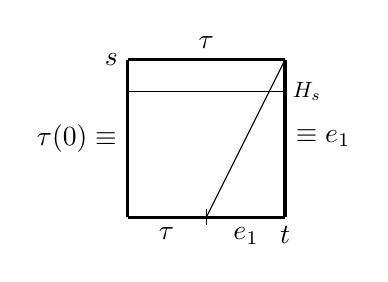
\begin{tikzpicture}[
				witharrow/.style={postaction={decorate}},
				vdot/.style={rectangle, fill, inner sep=0pt, outer sep=0pt, minimum width=0.5pt, minimum height=6pt}
				]
				
				\begin{scope}
				\draw[very thick]
				(0,0) coordinate (a1) -- node[left]{$\tau(0)\equiv$} (0,2) coordinate (d1)
				(2,0) coordinate (b1) -- node[right](q1){$\equiv e_1$} (2,2) coordinate (c1);
				
				\draw[very thick] (d1) -- node[above]{$\tau$} (2,2) coordinate (c1);
				
				\node[vdot] (b2) at (1,0) {};
				\draw[very thick] (a1) -- node[below]{$\tau$} (b2)
				(b2) -- node[below]{$e_1$} (b1);
				
				\draw[thin] (b2) -- (c1);
				
				\draw[very thin] (0, 1.6) -- (2,1.6) coordinate (h);
				\node[right, scale=0.8] at (h) {$H_s$};
				
				\node[below] at (b1) {$t$};
				\node[left] at (d1) {$s$};
				\end{scope}
				\end{tikzpicture}}
				
				\caption{Esquema de las homotopía para elementos neutros.}
			\end{figure}
		
			De nuevo, la intuición detrás de esta construcción es la misma. Es un buen ejercicio escribir las homotopías al detalle, y no lo haremos aquí. Además, el argumento de buena definición y continuidad es idéntico al del apartado anterior.
			
			\item En este caso, basta con demostrar que $\sigma\pathp\sigma' \homot e_0$ con extremos fijos, puesto que $\sigma=\sigma''$, y entonces aplicando el argumento a $\sigma'$ hemos terminado. Aunque la intuición geométrica es muy similar, la homotopía que resulta es algo distinta a los casos anteriores, y vamos a verla con algo más de detalle.
			
			Geométricamente, $\sigma'$ es $\sigma$ recorrido ``a la misma velocidad'', pero en sentido contrario. Entonces, $\sigma\pathp\sigma'$ va de $\sigma(0)$ a $\sigma(1)$ y vuelve por el mismo recorrido hasta $\sigma(0)$. Por tanto, la homotopía que vamos a considerar lo que hace es ``acercar cada vez más el punto donde se da la vuelta'', y esto en el extremo es una constante.
			
			\begin{figure}[h!]
				\label{grf_fig_homot_3}
				\centering
				\begin{tikzpicture}[
				decoration={markings,mark=at position 0.5 with {\arrow{>}}},
				witharrow/.style={postaction={decorate}},
				vdot/.style={rectangle, fill, inner sep=0pt, outer sep=0pt, minimum width=0.5pt, minimum height=6pt},
				dot/.style={draw,fill,circle,inner sep=1.5pt,minimum width=0pt, scale=0.45}
				]
				
				\begin{scope}
				\draw[very thick]
				(0,0) coordinate (a1) -- node[left]{$\sigma(0)\equiv$} (0,2) coordinate (d1)
				(2,0) coordinate (b1) -- node[right](q1){$\equiv\sigma'(1)$} (2,2) coordinate (c1);
				
				\draw[very thick] (d1) -- node[above]{$\sigma(0) = e_0$} (2,2) coordinate (c1);
				
				\node[vdot] (b3) at (1,0) {};
				\draw[very thick] (a1) -- node[below]{$\sigma$} (b3)
				(b3) -- node[below]{$\sigma\smash{'}$} (b1);
				
				\draw[thin] (b3) -- (d1);
				\draw[thin] (b3) -- (c1);
				
				\draw[very thin] (0, 1.5) -- (2,1.5) coordinate (h);
				\draw[thick] (0.25,1.5) coordinate (s1) -- (1.75,1.5) coordinate (s2);
				\node[dot] at (s1) {};
				\node[dot] at (s2) {};
				\node[above, scale=0.65] at (s1) {$\;\;\;\;\;\sigma(t)$};
				\node[above, scale=0.65] at (s2) {$\sigma(t)\;\;\;\;\;$};
				\node[right, scale=0.8] at (h) {$H_s$};
				
				\node[below] at (b1) {$t$};
				\node[left] at (d1) {$s$};
				\end{scope}
				\end{tikzpicture}
				
				\caption{Esquema de la homotopía entre $\sigma\pathp\sigma'$ y $e_0\equiv\sigma(0)$.}
			\end{figure}
		
			En este caso, la homotopía queda:
			\[H_s(t)=\left\{\begin{array}{ll}
			\sigma(2t) & \text{si } 0\leq t\leq\frac{1-s}{2} \\
			\sigma(1-s) & \text{si } \frac{1-s}{2}\leq t\leq\frac{1+s}{2} \\
			\sigma'(2t-1) & \text{si } \frac{1+s}{2}\leq t\leq 1
			\end{array}\right.\]
			y la prueba de que está bien definida y es homotopía coincide con la de los casos anteriores.
			
			\item En las condiciones del enunciado, supongamos que $H_s:\alpha\homot\sigma$ y $F_s:\beta\homot\tau$, ambas con extremos fijos. Entonces, podemos construir directamente la homotopía con extremos fijos $\alpha\pathp\beta\homot\sigma\pathp\tau$ como la siguiente:
			\[H_s(t)=\left\{\begin{array}{ll}
			H_s(2t) & \text{si } 0\leq t\leq\frac{1}{2} \\
			F_s(2t - 1) & \text{si } \frac{1}{2}\leq t\leq 0
			\end{array}\right.\]
			donde es interesante notar que se construye de forma muy similar al producto de dos caminos. Otra vez, la prueba de que está bien definida y es homotopía es la misma. \qedhere
		\end{enumerate}
	\end{proof}
\end{lem}

\section{Grupo fundamental}

Tras todas las preparaciones, por fin estamos en condiciones de afrontar el concepto que da nombre a este capítulo: el grupo fundamental.

No está de más recordar que $\X$ es, si no se dice lo contrario, conexo y localmente conexo por caminos.

\begin{defi}[Grupo fundamental]
	Sea $x_0\in\X$. Definimos el \tbi{grupo fundamental} de $\X$ con base $x_0$ como:
	\[\begin{split}
	\pi(\X,x_0) &= \left\{\text{lazos de base } x_0\right\} / {\homotef} \\
	&=\{\sigma:[0,1]\overset{\text{ cont.}}{\to}\X \mid \sigma(0)=\sigma(1)=x_0\} / {\homotef}
	\end{split}\]
	esto es, el conjunto de clases de homotopía de lazos, con la operación ${\pathp}$:
	\[\class{\sigma}\pathp\class{\tau} = \class{\sigma\pathp\tau}\]
\end{defi}

\begin{lem}
	El grupo fundamental está bien definido.
	
	\begin{proof}
	Hay que ver, primero, que la operación ${\pathp}$ está bien definida, y después que efectivamente es un grupo.
	
	Ya vimos en el lema \ref{grf_lema_prop_pathp} que la operación ${\pathp}$ respeta homotopía de extremos fijos, y por tanto la operacion ${\pathp}$ entre clases de equivalencia está bien definida.
	
	Entonces, solo queda ver que es un grupo. Hay que comprobar que es asociativa, que existe un elemento neutro y que todo elemento tiene inverso. Todas ellas se siguen de la propiedad correspondiente del lema \ref{grf_lema_prop_pathp}. Lo único que merece la pena comentar es que, en el caso del elemento neutro, el hecho de restringir los caminos a lazos con un punto base común garantiza la unicidad, y este elemento neutro es precisamente $x_0$.
	\end{proof}
\end{lem}

\begin{exa}[Grupos fundamentales]
	Presentamos ahora una serie de ejemplos de grupos fundamentales. Muchos de ellos los iremos demostrando a lo largo del texto, aunque habrá algunos que no lleguemos a ver por su complicación.
	
	Nótese que a menudo omitimos el punto base, porque, como veremos pronto, los grupos fundamentales para el mismo espacio respecto de distintos puntos base son isomorfos.
	
	\begin{enumerate}
		\item Dado $\X\subset\R^n$ estrellado, si tomamos como punto base el $x_0$ del ``centro'', ya vimos en el ejemplo \ref{grf_nulhomotopias_convexos} que todas las funciones son nulhomótopas, y entonces:
		\[\pi(\X,x_0)=\{1\}\]
		
		\item También vimos, en la proposición \ref{grf_homotop_caminos_esfera}, que $\pi(\Sfe^n)=\{1\}$ si $n\geq 2$.
		
		\item Para $n=1$, la circunferencia, resulta que $\pi(\Sfe^1)=\Z$.
		
		\item Un ejemplo de espacio con grupo fundamental finito no trivial es el espacio proyectivo real: $\pi(\proy^n)=\Z_2$.
		
		\item Como veremos más adelante, el producto de espacios tiene como grupo fundamental el producto de los grupos. Entonces, $\pi(\toro)=\pi(\Sfe^1)\times\pi(\Sfe^1)=\Z^2$.
		
		\item Para $\toro_g$, el toro con $g$ agujeros, tenemos que existe un homomorfismo de grupos sobreyectivo $\pi(\toro_g)\twoheadrightarrow \Z^2$. De hecho, en general, $\pi(\toro_g)$ ni siquiera es abeliano.
		
		\item El grupo fundamental del bouquet $B_n$, una figura geométrica generada pegando $n$ circunferencias, es $\pi(B_n)=\Z\pathp\overset{n}{\dots}\pathp\Z$, donde ${\pathp}$ denota el producto libre de grupos. Más adelante entraremos en detalle en este tema.
		
		\begin{figure}[h!]
			\centering
			\begin{tikzpicture}[scale = 0.4]
			\begin{polaraxis}[grid=none, axis lines=none]
			\addplot[mark=none,domain=0:360,samples=300] {cos(x*3)};
			\end{polaraxis}
			\end{tikzpicture}
			
			\caption{Un bouquet de tres pétalos.}
		\end{figure}
	
		\item $\pi(\Sfe^2\times\Sfe^2)=\{1\}$ y $\pi(\Sfe^4)=\{1\}$ pero $\Sfe^2\times\Sfe^2\centernot\homeo\Sfe^4$. Esto, que parece ser un contraejemplo a la versión generalizada para $n=4$ de la conjetura de Poincaré (\ref{grf_conjet_poincare}), no es tal; ya que para $n\geq 4$ se formula con condiciones adicionales. \qedhere
	\end{enumerate}
\end{exa}

\begin{prop}
	El grupo fundamental es independiente del punto base. Es decir, si $x_0,x_1\in\X$, entonces $\pi(\X,x_0)$ y $\pi(\X,x_1)$ son isomorfos.
	
	\begin{proof}
		Como asumimos que $\X$ es conexo por caminos, entonces existe un camino de $x_0$ a $x_1$ que llamamos $\alpha$. Así, definimos la siguiente función:
		\[\begin{split}
		f:\pi(\X,x_0) &\to \pi(\X,x_1) \\
		[\sigma]&\mapsto [\alpha'\pathp\sigma\pathp\alpha]
		\end{split}\]
		
		Y queremos comprobar que es isomorfismo de grupos:
		\begin{enumerate}
			\item Desde luego, está bien definida (si dos caminos son homótopos con extremos fijos, multiplicarlos por $\alpha$ y $\alpha'$ conserva la homotopía). Nótese que siguen siendo homótopos por extremos fijos pero los extremos en sí son otros,
			
			\item Es homomorfismo de grupos. En efecto, queremos ver que la imagen del producto es el producto de las imágenes. Entonces:
			\[f([\sigma]\pathp[\tau]) = f([\sigma\pathp\tau])=[\alpha'\pathp\sigma\pathp\tau\pathp\alpha]=[\alpha'\pathp\sigma\pathp\alpha\pathp\alpha'\pathp\tau\pathp\alpha] = [\alpha'\pathp\sigma\pathp\alpha]\pathp[\alpha'\pathp\tau\pathp\alpha=f([\sigma])\pathp f([\tau])\]
			
			\item Es isomorfismo, porque su inversa es $[\lambda]\mapsto[\alpha\times\lambda\times\alpha']$ y esto es, por el apartado anterior, un homomorfismo. \qedhere
		\end{enumerate}
	\end{proof}
\end{prop}

\begin{obs}
	La proposición anterior parece dejar resuelto todo lo relativo al punto base: no solo nos garantiza que el grupo fundamental es independiente del punto base sino que además nos proporciona un isomorfismo explícito. Sin embargo, hay que tener cuidado con esto. Si pretendemos identificar todos los grupos fundamentales con uno solo, nos encontramos una dificultad: el isomorfismo depende del camino que escojamos. No hay una forma canónica de identificar uno por otro. 
	
	No es incorrecto hablar \ti{del} grupo fundamental de un espacio, pero siempre hay que tener en mente la consideración anterior. Como curiosidad, si el grupo fundamental es abeliano el isomorfismo sí es independiente del camino. 
\end{obs}

\begin{obs}
	Nótese que hemos necesitado que el espacio sea conexo por caminos para llevar a cabo la prueba anterior. Este es, de hecho, uno de los principales motivos por los que hemos restringido de tal forma el espacio $\X$.
\end{obs}

Para terminar la sección, definimos un concepto que nos ayudará a tratar con espacios con grupo fundamental trivial.

\begin{defi}[Simplemente conexo]
	Decimos que un espacio $\X$ conexo por caminos es \tbi{simplemente conexo} cuando su grupo fundamental es trivial.
\end{defi}

\section{\ti{General nonsense}. Funtorialidad}

El objetivo principal de esta sección es aplicar las ideas de teoría de categorías a los conceptos que hemos ido viendo a lo largo de este capítulo. Así, se recomienda leer antes el anexo \ref{funt}, que contiene una brevísima introducción a los conceptos más básicos de teoría de categorías. Esta no solo define los conceptos básicos como categoría o funtor sino que puede ayudar al lector a comprender el propósito detrás de este punto de vista, que a primera vista puede parecer terriblemente abstracto.

\begin{const}[Interpretación funtorial del grupo fundamental]
	En esta sección, vamos a considerar dos categorías. La primera de ellas es la \index[general]{categoría}categoría de espacios topológicos punteados \Topp, cuyos objetos son: 
	\[\{((\X,\T),x_0)\midc (\X,\T)\text{ espacio topológico}, x_0\in\X\}\]
	y en la cual los morfismos son las funciones continuas que preservan el punto base $x_0$. La segunda de ellas la categoría de los grupos \Grp, que tiene por objetos:
	\[\{(G,\cdot)\midc (G,\cdot) \text{ grupo}\}\]
	y por morfismos los homomorfismos de grupos.
	
	Entonces, consideramos tomar el grupo fundamental como un \index[general]{funtor}funtor. Es decir, consideramos el funtor $\pi$:
	\[\xymatrix @R=0.5pc @C=0.5pc {
		& & \Topp \ar[rrr]^\pi & & & \Grp & \\
		& & (\X,x_0) \ar@{|->}[rrr] \ar[dd]_{f \text{ cont.}} \ar@<1.5ex>@{|->}[dd] & & & \pi(\X,x_0) \ar[dd]_{f^\ast}^{\text{homom.}} \ar@{}[r]|-\ni & [\sigma] \ar@{|->}[dd] \\
		[0,1] \ar[urr]^\sigma \ar[drr]_{f\circ\sigma} & & & & & & \\
		& & (\Y,y_0) \ar@{|->}[rrr] & & & \pi(\Y,y_0) \ar@{}[r]|-\ni & [f\circ\sigma] \\
	}\]
	Nótese que denotamos $f^\ast$ al homomorfismo de grupos que es imagen de una aplicación continua $f$ por el funtor $\pi$.
	Como se aprecia en el diagrama, este homomorfismo $f^\ast$ se define, para una clase de equivalencia de caminos, de la siguiente forma:
	\[\begin{split}
	f^\ast:(\X, x_0) &\to (\Y, y_0) \\
	[\sigma] &\mapsto [f\circ\sigma]
	\end{split}\]
	Hay que comprobar, entonces, que está bien definido. En efecto, consideramos la aplicación $f^\ast$ que acabamos de definir. Desde luego, si $\sigma$ es un lazo con base $x_0$, $f\circ\sigma$ es un lazo con base $y_0$. Para ver si respeta la homotopía, consideramos $\tau:[0,1]\to (\X,x_0)$ homótopo con extremos fijos con $\sigma$ a través de la homotopía $H$. Entonces, $f\circ H$ es una homotopía entre $f\circ\sigma$ y $f\circ\tau$. Por último, comprobamos que es homomorfismo, lo cual es directo comprobando que $f\circ(\sigma\ast\tau)=(f\circ\sigma)\ast (f\circ\tau)$.
	
	Además, hay que ver que es un funtor, esto es, que cumple:
	\begin{itemize}
		\item $(g\circ f)^\ast = g^\ast\circ f^\ast$. En efecto, consideramos el lazo $\sigma$ con base en $x_0$. Sabemos que:
		\[(g\circ f)\circ\sigma=g\circ(f\circ\sigma)\]
		y tomando la imagen de $\sigma$ por $(g\circ f)^\ast$:
			\[(g\circ f)^\ast([\sigma])=[(g\circ f)\circ\sigma]=[g\circ(f\circ\sigma)]=g^\ast([f\circ\sigma])=g^\ast(f^\ast([\sigma]))\]
		como queríamos comprobar.
		
		\item $(\Id_\X)^\ast = \Id_{\pi(\X, x_0)}$. Esto se verifica directamente por como hemos definido $f^\ast$.
	\end{itemize}
\end{const}

Visto todo lo necesario, podemos pasar a comprobar una serie de propiedades utilizando el punto de vista introducido en la construcción anterior. La teoría de categorías es capaz a menudo de simplificar demostraciones al considerar los objetos abstractos, lo cual es una de sus grandes fortalezas. Vamos a ver ahora una serie de proposiciones que al mismo tiempo son ejemplos, pues muestran como enfocaríamos una demostración desde este nuevo punto de vista. Sin embargo, no dejan de ser resultados interesantes por sí mismos.

\begin{prop}
	El funtor grupo fundamental manda homeomorfismos en isomorfismos de grupos. En particular, si dos espacios tienen distinto grupo fundamental, entonces no son homeomorfos.
	
	\begin{proof}
		Sean $\X,\Y$ dos espacios topológicos punteados con $x_0$, $y_0$, y $f$ un homeomorfismo entre ellos de forma que:
		\[\xymatrix @R=0.4pc {
			\X \ar[r]^f_{\text{homeo.}} & \Y \ar[r]^{g=f^{-1}} & \X \\
			x_0 \ar@{|->}[r] & y_0 \ar@{|->}[r] & x_0
		}\]
		
		Ahora, tenemos que:
		\[g^\ast\circ f^\ast = (g\circ f)^\ast = (\Id_\X)^\ast = \Id_{\pi(X)}\]
		\[f^\ast\circ g^\ast = (f\circ g)^\ast = (\Id_\Y)^\ast = \Id_{\pi(Y)}\]
		y con esto hemos comprobado que $g^\ast$ es la inversa de $f^\ast$, luego $f^\ast$ es isomorfismo.
	\end{proof}
\end{prop}

\begin{prop}
	\label{grf_prop_retractos_homo_sobreyectivo}
	Un \index[general]{retracto}retracto, como veremos con detalle más adelante, es un subespacio tal que existe una aplicación continua que deforma el espacio en él, como se aprecia en el siguiente esquema:
	\[\xymatrix @C=0.65pc {
		A \ar@{}[r]|\subset \ar[dr]_{\rho\restriction_A = \Id} & \X \ar[d]^{\rho\text{ retracto}} \\
		& A
	}\]
	Entonces, la imagen $\rho^\ast$ de $\rho$ por $\pi$ es un homomorfismo sobreyectivo. En particular, si el grupo fundamental del retracto $A$ es no trivial, entonces el grupo fundamental del espacio $\X$ tampoco es trivial.
	
	\begin{proof}
		Para la demostración, consideramos la imagen por $\pi$ del diagrama anterior, donde $A$ y $\X$ tienen el mismo punto base $x_0\in A$:
		\[\xymatrix {
			\pi(A,x_0) \ar[r]^{j^\ast} \ar[dr]_{(\rho\restriction_A)^\ast = \Id_{\pi(A)}} & \pi(\X,x_0) \ar[d]^{\rho^\ast} \\
			& \pi(A,x_0)
		}\]
		donde $j$ es la aplicación inclusión de $A$ en $\X$. Como por las propiedades de los funtores $\rho^\ast\circ j^\ast=(\rho\circ j)^\ast$, el diagrama anterior conmuta, es decir:
		\[\rho^\ast\circ j^\ast=\Id_{\pi(A)}\]
		
		Ahora, como $\Id_{\pi(A)}$ es biyectivo, y en particular sobreyectivo, $\rho^\ast\circ j^\ast$ también debe ser sobreyectivo, y entonces necesariamente $\rho^\ast$ lo es.
	\end{proof}
\end{prop}

Un caso donde se puede aplicar la proposición anterior es el siguiente.

\begin{exa}
	Consideramos el disco cerrado $\adher{D}_2\subset\R^2$. Queremos comprobar que el disco no se puede retraer a $A=\Sfe^1=\partial\adher{D}_2$. Como veremos más adelante, $\pi(A)=\pi(\Sfe^1)=\Z$, y ya sabemos que $\pi(\adher{D}_2)=\{1\}$, pues es un estrellado en $\R^n$. Entonces, si fuera retracto, habría un homomorfismo sobreyectivo del grupo trivial a $\Z$, y esto es imposible.
\end{exa}

\begin{prop}
	\label{grf_prop_gf_prod_es_prod_gf}
	Dados dos espacios $\X,\Y$, el grupo fundamental del producto es isomorfo al producto de los grupos fundamentales. Esto es:
	\[\pi(\X\times\Y)\approx\pi(\X)\times\pi(\Y)\]
	
	\begin{proof}
		Consideramos los puntos base $x_0,y_0$ respectivamente. El esquema de la topología producto sería el siguiente:
		\[\xymatrix @R = 0.4pc{
			& \X & \\
			\X\times\Y \ar[ur]^p \ar[dr]_q & & [0,1] \ar[ul]^\sigma \ar[dl]^\tau \\
			& \Y &
		}\]
		donde $p$ y $q$ son las proyecciones. Entonces, como ya hemos hecho antes, vamos a ver la imagen de este diagrama:
		\[\xymatrix @R = 0.4pc @C = 0.5pc {
			& \pi(\X) & & & *+[r]{[p\circ (\sigma,\tau)]=[\sigma]} \\
			\pi(\X,\Y)  \ar[ru]^{p^\ast} \ar[rd]_{q^\ast} \ar[rr]^-{(p^\ast,q^\ast)} & & \pi(\X)\times\pi(\Y) \ar@{}[r]|-\colon& [(\sigma,\tau)] \ar@{|->}[ru] \ar@{|->}[rd] \ar@{|->}[r] & ([\sigma],[\tau]) \\
			& \pi(\Y) & & & *+[r]{[q\circ (\sigma,\tau)]=[\tau]}
		}\]
		
		Nótese que hemos añadido la aplicación que llega a $\pi(\X)\times\pi(\Y)$. Si comprobamos que es un isomorfismo, entonces tenemos lo que estábamos buscando. En efecto:
		\begin{itemize}
			\item Es trivialmente sobreyectivo.
			\item Es inyectivo. Para verlo, usaremos un resultado conocido que afirma que un homomorfismo es inyectivo si y solo si su núcleo es trivial. Entonces, denotando $e_X$ al elemento identidad de cada grupo $\pi(X)$, sean $\sigma,\tau$ de forma que $([\sigma],[\tau])=(e_\X,e_\Y)$. Queremos ver que necesariamente $[(\sigma,\tau)]=e_{\X\times \Y}$.
			
			Consideramos las homotopías $K_s:\sigma\homot x_0=e_\X$, $L_s:\tau\homot y_0=e_\Y$. Entonces, $(K_s,L_s):(\sigma,\tau)\homot(x_0,y_0)=e_{\X\times\Y}$ es homotopía y, por tanto, el núcleo del homomorfismo es $\{e_{\X\times\Y}\}$.
		\end{itemize}
		Por tanto, es isomorfismo.
	\end{proof}
\end{prop}

Un ejemplo de la utilidad de este resultado es el siguiente.

\begin{exa}
	Consideramos el toro $\toro$, que sabemos que es homeomorfo a $\Sfe^1\times\Sfe^1$. Entonces, cuando veamos más adelante que $\pi(\Sfe^1)=\Z$, podremos afirmar directamente que $\pi(\toro)=\Z\times\Z$.
\end{exa}

\section{Espacios recubridores. El problema de elevación}

El estudio de los espacios recubridores de otro espacio es a menudo útil para calcular grupos fundamentales, y en general tiene una gran relación con el estudio de ellos. En esta sección planteamos el problema de elevación en su versión más general, para luego particularizarlo para poder demostrar propiedades útiles.

\subsection{Espacios recubridores}

Para empezar, vamos a formalizar el concepto de espacio recubridor.

\begin{defi}[Espacio recubridor]
	Sea $p:\widetilde{\X}\to \X$ una aplicación continua y sobreyectiva. Decimos que $\widetilde{\X}$ es un \tbi[espacio!recubridor]{espacio recubridor} de $X$ si para cada $x\in\X$ existe un entorno $U_x$ que verifica que $p^{-1}(U_x)$ se puede escribir como unión disjunta de conjuntos $U_\lambda$ donde cada uno de ellos es homeomorfo a $U_x$, de forma que, para cada $\lambda$, $p\restriction_{U_\lambda}:U_\lambda\to U_x$ sea un homeomorfismo.
\end{defi}

\begin{exa}[Recubrimientos]
	\label{grf_exa_recubrimientos}
	Veamos algunos ejemplos de espacios recubridores.
	
	\begin{enumerate}
		\item $\Sfe^n$ recubre al plano proyectivo real $\proy^n$, con la siguiente aplicación:
		\[\begin{split}
		p:\Sfe^n&\to\proy^n \\
		(x_0,\dots,x_n)&\mapsto (x_0:\dotsc:x_n)
		\end{split}\]
		En efecto, tomamos un punto $(x_0:\dotsc:x_n)\in\proy^n$. Tomando un entorno abierto del punto, homeomorfo a un disco, su imagen inversa consiste en dos abiertos homeomorfos a discos alrededor de dos puntos antipodales de $\Sfe^n$. Estos son disjuntos y se verifican las condiciones.
		
		\item $\R$ recubre al círculo $\Sfe^1$, con la aplicación:
		\[\begin{split}
		p:\R&\to\Sfe^1 \\
		t &\mapsto e^{2\pi t}=(\cos 2\pi t,\sin 2\pi t)
		\end{split}\]
		En efecto, para un punto $x$ del círculo, tomamos un entorno abierto: un arco que lo contenga sin extremos. Esto es homeomorfo a un intervalo abierto, y su imagen inversa consiste en una cantidad numerable de intervalos a lo largo de la recta real, cada uno conteniendo un punto de $p^{-1}(x) = \Z + a$ para algún $a\in\R$. Como, tomando el entorno inicial lo suficientemente pequeño, todos estos intervalos son disjuntos, ya está. \qedhere
	\end{enumerate}
\end{exa}

\subsection{El problema de elevación}

Con esto, estamos ya en condiciones de formular el problema de elevación.

\begin{const}[Formulación del problema de elevación]
	\index[general]{problema de elevación}
	Consideramos el diagrama:
	\[\xymatrix{
		& \widetilde{\X} \ar[d]^p \\
		\mc{Z} \ar@{-->}[ru]^{\widetilde{H}} \ar[r]^H & \X
	}\]
	
	Aquí, $\widetilde{\X}$ es un espacio recubridor mediante la aplicación $p$. El problema de elevación pregunta por la existencia de la aplicación del diagrama $\widetilde{H}:\mc{Z}\to\X$, continua y que verifique que $p\circ\widetilde{H}=H$, es decir, que haga que el diagrama sea conmutativo. Una aplicación que verifique esto se llama \tbi{elevación}.
\end{const}

\begin{lem}[Existencia de elevación local]
	\label{grf_lema_elevacion_local}
	Sea $z_0\in\mc{Z}$, $x_0=H(z_0)\in U$ abierto de $\X$. Entonces, para un único $\lambda$, existe una elevación local $\widetilde{H}$ que muere en $U_\lambda$ de forma que el siguiente esquema es conmutativo:
	\[\xymatrix{
		& U_\lambda \ar[d]^{p\restriction_{U_\lambda}} \\
		\mc{Z}\supset H^{-1}(U) \ar[ru]^-{\widetilde{H}} \ar[r]^-H & U
	}\]

	Además, $\widetilde{H}=(p\restriction_{U_\lambda})^{-1}\circ H$.
	
	\begin{proof}
		Basta con comprobar que $\widehat{H}=(p\restriction_{U_\lambda})^{-1}\circ H$ es una elevación, bien definida, que muere en $U_\lambda$. 
		
		Ahora, para ver que es elevación, basta con darse cuenta de que $p\restriction_{U_\lambda}$ es un homeomorfismo por definición de espacio recubridor. Entonces, no solo está bien definida (por existir la inversa de $p\restriction_{U_\lambda}$), sino que además la composición $\widetilde{H} = (p\restriction_{U_\lambda})^{-1}\circ H$ es continua y como, desde luego, hace conmutativo el diagrama, es elevación.
		
		Para ver que, en efecto, muere en $U_\lambda$, usamos que $\widetilde{H}(x_0)\in p^{-1}(x_0)$, pues $p\widetilde{H}(z_0)=H(z_0)=x_0$. Entonces, consideramos:
		\[\widetilde{H}(z_0)\in p^{-1}(x_0)\subset p^{-1}(U)=\bigcup_\lambda U_\lambda\]
		y como la unión es disjunta, existe un único $\lambda$ de forma que $\widetilde{H}(z_0)\in U_\lambda$.
	\end{proof}
\end{lem}

\begin{lem}[Unicidad de la elevación]
	\label{grf_lema_unicidad_elevacion}
	Si, para un $\mc{Z}$ conexo, dos elevaciones coinciden en un punto, entonces son la misma.
	
	\begin{proof}
		Consideramos dos elevaciones $\Phi$ y $\Psi$ que cumplan las condiciones anteriores. Queremos ver que ambas son la misma. Como $\mc{Z}$ es conexo, podemos comprobar que $\{\Phi(z)=\Psi(z)\}$, que es no vacío (porque, por hipótesis, coinciden en un punto), es abierto y cerrado en $\mc{Z}$.
		
		\begin{itemize}
			\item Veamos que es abierto. Sea $z\in\mc{Z}$, entonces existe un entorno $W$ de $z$ tal que $\Phi\restriction_{W}=(p\restriction_{U_\lambda})^{-1}\circ H$, y existe otro entorno $W'$ de $z$ tal que $\Psi\restriction_{W'}=(p\restriction_{U_\lambda})^{-1}\circ H$; con $\Phi(z)\in U_\lambda$ y $\Psi(z)\in U_\mu$. Como $\Phi(z)=\Psi(z)$, $U_\lambda = U_\mu$ (por ser la unión disjunta). Entonces $\Phi\restriction_{W\cap W'}=\Psi\restriction_{W\cap W'}$, y por tanto $W\cap W'\subset\{\Phi(z)=\Psi(z)\}$, y es entorno, luego este es abierto.
			
			\item Vamos a ver que el complementario $\{\Phi(z)\neq\Psi(z)\}$ es abierto. Primero, $\lambda\neq\mu$. En efecto, si estuvieran en el mismo $U_\lambda$, $p\Phi(z)\neq p\Psi(z)$, pero por ser elevaciones ambos son iguales a $H(z)$, lo cual es una contradicción. Entonces, si $\lambda\neq\mu$, definiendo $W$ y $W'$ como en el apartado anterior, $\Phi(W\cap W')\cap \Psi(W\cap W')\subset U_\lambda\cap U_\mu=\emptyset$. Entonces, $W\cap W'\subset \{\Phi(z)\neq\Psi(z)\}$, luego este es abierto. \qedhere
		\end{itemize}
	\end{proof}
\end{lem}

El lema que sigue tiene una importancia capital a la hora de demostrar cuál es el grupo fundamental de muchos espacios.

\begin{lem}[De elevación de homotopías]
	\label{grf_lema_elevacion_homotopias}
	Dada una homotopía $H:\mc{Z}=\Y\times [0,1]\to\X$ y una elevación $\widetilde{f}$ de $f=H_0:\Y\to\X$, entonces existe una única elevación $\widetilde{H}$ de $H$ tal que $(\widetilde{H})_0=\widetilde{f}$.
	
	\begin{proof}
		Nótese que no tenemos que preocuparnos de la unicidad: ya la demostramos en el lema \ref{grf_lema_unicidad_elevacion}. Será más complicado probar la existencia.
		
		La demostración de la existencia tiene dos pasos. Primero, trataremos de construir una elevación semilocal para luego intentar pegar todos estos ``trozos'' de elevación, construyendo así la elevación global. Recordamos de nuevo que estamos intentando construir una elevación que haga conmutativo el diagrama:
		\[\xymatrix{
			& \widetilde{\X} \ar[d]^p \\
			\Y\times [0,1] \ar@{-->}[ru]^{\widetilde{H}} \ar[r]^-H & \X
		}\]
		y que además verifique que $(\widetilde{H})_0=\widetilde{f}$.
		
		Vamos a construir, pues, lo que hemos llamado una elevación semilocal, es decir, para cada $y\in\Y$ una elevación $\widetilde{H}_y:V_y\times [0,1]\to\widetilde{X}$, donde $V_y$ es un entorno abierto de $\Y$.
		
		De esta forma, fijando $y\in \Y$, consideramos la restricción de $H$:
		\[\{y\}\times [0,1]\overset{H}{\to}X=\bigcup_x U_x\]
		Ahora, aplicamos el lema de Lebesgue (\ref{comp_lem_lebesgue}), considerando el recubrimiento abierto $H^{-1}(U_{x_i})$. Entonces, existe una partición $0=t_0<t_1<\dots<t_r=1$ de forma que $\{y\}\times [t_{i-1}, t_i]\subset H^{-1}(U_{x_i})\subset \Y\times [0,1]$ para ciertos $x_i$. Aplicando el conocido lema de Wallace (que no hemos demostrado aquí), como $H^{-1}(U_{x_i})$ es un abierto en el compacto $\Y\times [0,1]$, y $\{y\}\times [t_{i-1},t_i]$ es un compacto en ese abierto, entonces existe un entorno $V_y^i$ de forma que $V_y^i\times [t_{i-1},t_i]\subset H^{-1}(U_{x_i})$. Entonces, definimos $V_y=\bigcap_{j=1}^r V_y^j$ entorno abierto de $y$.
		
		Con el entorno definido de esta forma, vamos a fabricar la elevación $\widetilde{H}_y$ de $H\restriction_{V_y\times [0,1]}$. Para ello, vamos a considerar, para cada $i$, la restricción $H:V_y^i\times [t_{i-1},t_i]\to U_{x_i}$. Procedemos por inducción sobre los $\{t_0,\dots, t_r\}$ de la partición:
		
		\begin{itemize}
			\item El caso base es simplemente la homotopía:
			\[\widetilde{H}_y\restriction_{V_y\times\{0\}}=\widetilde{f}\restriction_{V_y}\]
			
			\item Para el paso inductivo, supongamos dada $\widetilde{H}_y\restriction_{V_y\times [0,t_i]}$. Como se cumple que la homotopía $H\restriction_{V_y\times [t_i,t_{i+1}]}$ acaba en $U^{x_{i+1}}$, resulta que $H(y,t_i)\in U_{x_{i+1}}$. Entonces, se cumple:
			\[\widetilde{H}^y(y, t_i)\in p^{-1}(U^x_{i+1})=\bigcup_\lambda U_\lambda^{x_{i+1}}\]
			donde la unión es disjunta. De esta forma, existe un (único) $\lambda$ tal que $\widetilde{H}_y(y, t_i)\in U_\lambda^{x_{i+1}}$. Así, $(y,t_i)\in (\widetilde{H}_y)^{-1}(U_\lambda^{x_{i+1}})$, que es abierto, y por tanto existe un entorno $W_y$ que cumple que $W_y\times \{t_i\}\subset (\widetilde{H}_y)^{-1}(U_\lambda^{x_{i+1}})$. Reducimos entonces el entorno original $V_y$ a $V_y\cap W_y$, que desde luego es entorno por ser intersección de entornos, y entonces $V_y\times\{t_i\}\subset (\widetilde{H}_y)^{-1}(U_\lambda^{x_{i+1}})$.
			
			Ahora, por el lema \ref{grf_lema_elevacion_local} de elevación local, ya que tenemos que:
			\[V_y\times [t_i, t_{i+1}]\subset H^{-1} U^{x_{i+1}}\]
			podemos encontrar una elevación:
			\[\widetilde{H}_y\restriction_{V_y\times [t_i,t_{i+1}]} = (p\restriction_{U_\lambda^{x_{i+1}}})^{-1}\circ H \]
			
			Con lo anterior, solo necesitamos comprobar que la aplicación:
			\[\widetilde{H}_y\restriction_{V_y\times [0,t_{i+1}]} = \left\{\begin{array}{ll}
			\widetilde{H}_y\restriction_{V_y\times [0,t_i]} & \text{si } 0\leq t \leq t_i \\
			\widetilde{H}_y\restriction_{V_y\times [t_i,t_{i+1}]} & \text{si } t_i\leq t \leq t_{i+1} \\
			\end{array}\right.\]
			está bien definida, es continua y es elevación. 
			
			Que está bien definida se ve rápidamente a partir de las comprobaciones anteriores. En efecto, hay que comprobar que el valor de cada trozo en $V_y\times\{t_i\}$ coincide. Para ello, usaremos que ambas son elevaciones de $H$, de forma que, para cualquier $y'\in V_y$:
			\[p\restriction_{U_\lambda^{x_{i+1}}}(\widetilde{H}_y\restriction_{[0,t_i]}(y',t_i)) = H(y',t_i) = p\restriction_{U_\lambda^{x_{i+1}}}(\widetilde{H}_y\restriction_{[t_i,t_{i+1}]}(y',t_i)) \]
			y por ser $p\restriction_{U_\lambda^{x_{i+1}}}$ homeomorfismo son iguales.
			
			La continuidad es directa por existir un recubrimiento cerrado tal que la restricción es continua en cada parte (los propios trozos). Y que es elevación se comprueba directamente.
		\end{itemize}
	
		Con esta inducción, hemos generado, para cada $y\in\Y$, una elevación $\widetilde{H}_y:V_y\times [0,1]\to\widetilde{X}$. Ahora, pasamos a ver que se pueden ``pegar'' todas estas elevaciones para construir una elevación global. 
		
		Consideramos pues dos puntos $y,y'\in\Y$ y las elevaciones correspondientes $\widetilde{H}_y$ y $\widetilde{H}_{y'}$. Basta comprobar que ambas coinciden el la parte común de los dominios: $V_y\cap V_{y'}$.
		
		Para probar esto, consideramos $y''\in V_y\cap V_{y'}$. Queremos comprobar que $\widetilde{H}_y(y'',\cdot)=\widetilde{H}_{y'}(y'',\cdot)$. Pero ambas son elevaciones de $H$ en $\{y''\}\times [0,1]$ y entonces ambas deben cumplir:
		\[\widetilde{H}_y(y'',0)=\widetilde{f}(y'')=\widetilde{H}_{y'}(y'',0)\]
		
		Entonces, como coinciden en un punto de un conexo ($\{y''\}\times [0,1]$), ya vimos en el lema \ref{grf_lema_unicidad_elevacion} que coinciden. 
	\end{proof}
\end{lem}

El siguiente resultado bien podría llamarse corolario, pues es un caso particular del lema de elevación de homotopías, pero dada la importancia que tiene lo consideramos un lema en sí mismo.

\begin{lem}[De elevación de caminos]
	\label{grf_lema_elevacion_caminos}
	Dado un camino $\sigma:\mc{Z}= [0,1]\to\X$, de origen $x_0\in\X$, entonces existe una única elevación $\widetilde{\sigma}$ de $\sigma$ tal que el origen de $\widetilde{\sigma}$ sea $\widetilde{x_0}\in\widetilde{X}$.
	
	\begin{proof}
		Si en el lema de elevación de homotopías tomamos $\Y=\{a\}$, y consideramos la función $\widetilde{f}:\Y\to \widetilde{\X}$ tal que $\widetilde{f}(a)=\widetilde{x_0}$, tenemos el resultado.
	\end{proof}
\end{lem}

\begin{obs}
	La elevación es un problema homotópico. En efecto, si $f:\Y\to\X$ tiene una elevación $\widetilde{f}:\Y\to\widetilde{\X}$, entonces toda $g\homot f$ tiene también elevación.  Basta con considerar la homotopía $H:f\homot g$, y por el lema de elevación existe $\widetilde{H}$, de forma que $\widetilde{g} = \widetilde{H}_1$ eleva a $g$.
\end{obs}

\section{El grupo fundamental del espacio proyectivo}

El objetivo de esta sección es calcular el grupo fundamental de $\proy^n$, el espacio proyectivo real de dimensión $n$, para $n\geq 2$. Como pronto veremos, esta demostración explota el concepto de elevación. 

\begin{theo}[Grupo fundamental de $\proy^n$]
	\label{grf_espacio_proyectivo}
	
	Para $n\geq 2$, el grupo fundamental de \indexg{espacio proyectivo} $\proy^n$ es $\pi(\proy^2)=\Z_2$, el grupo abeliano de orden 2.
	
	\begin{proof}
		Vamos a empezar demostrando que la esfera $\Sfe^n$ es un espacio recubridor del espacio proyectivo $\proy^n$. Vamos a repetir con un poco más de detalle el argumento que ya utilizamos en el ejemplo \ref{grf_exa_recubrimientos}. Consideramos pues la aplicación:
		\[\begin{split}
		p:\Sfe^n&\to\proy^n \\
		(x_0,\dots,x_n)&\mapsto (x_0,\dotsc,x_n)
		\end{split}\]
		Entonces, sea un punto $y\in\proy^n$. Tenemos que comprobar que para cada $x\in p^{-1}(y)$ existe un entorno $U_x$ tal que $p^{-1}(U_x)$ es union disjunta de conjuntos $U_\lambda$, donde cada $U_\lambda\homeo U_x$.
		
		De esta forma, para $y\in\proy^n$, consideramos un hiperplano $\pi$ que no lo contenga. Como el plano $\pi$ es cerrado, $U=\proy^n\setminus\pi$ es abierto, y además contiene a $x$, luego es entorno. La imagen inversa del plano $\pi$ es, para la misma aplicación definida en todo $\R^{n+1}$, un hiperplano; y de esta manera la imagen inversa de $\proy^n\setminus\pi$ por $p:\Sfe^n\to\proy^n$ son dos casquetes de la esfera. Llamamos pues a estos $U_+$, $U_-$ y desde luego son abiertos. Como la imagen inversa de $x$ son dos puntos antipodales, que llamamos $p$ y $-p$, y no están en $p^{-1}(\pi)$, entonces está cada uno en un casquete. De esta forma, como los casquetes son entornos disjuntos, basta con comprobar que $U_+,U_-\homeo U_x$. Pero resulta que $U_x = \proy^n\setminus\pi\homeo\R^n$, y $U_+,U_-\homeo\R^n$ porque son homeomorfos a discos abiertos.
		
		Visto esto, planteamos la siguiente elevación de caminos. Sea $a=(1:0:\dotsc:0)$ el punto base del grupo fundamental. Entonces, tenemos el diagrama:
		\[\xymatrix @C = 0.5pc {
			&& \Sfe^n \ar[d]^p & (x_0,\dots,x_n) \ar@{|->}[d] \ar@{}[l]|-\ni \\
			[0,1] \ar[rr]^\sigma \ar[rru]^{\widetilde{\sigma}} && \proy^n & (x_0,\dotsc,x_n) \ar@{}[l]|-\ni
		}\]
		de forma que $\sigma$ es un lazo en $\proy^n$ con base en $a$, y por tanto verifica $\sigma(0)=\sigma(1)=a$. Si llamamos $p^{-1}(a)=\{\widetilde{a},-\widetilde{a}\}$, por el lema de elevación de caminos (\ref{grf_lema_elevacion_caminos}), podemos elegir $\widetilde{\sigma}$ de forma que se verifique que $\widetilde{\sigma}(0)=\widetilde{a}$. Pero como tan solo sabemos que $p\circ\widetilde{\sigma}=\sigma$, entonces $\widetilde{\sigma}(1)$ no tiene por qué ser $\widetilde{a}$, puede ser también $-\widetilde{a}$.
		
		Planteamos entonces dos casos:
		\begin{enumerate}[label=\roman*]
			\item $\widetilde{\sigma}$ es un lazo en $\Sfe^n$ de base $\widetilde{a}$. Como ya vimos en la proposición \ref{grf_homotop_caminos_esfera} que $\pi(\Sfe^n)=\{1\}$, podemos escribir:
			\[\widetilde{H}_s:\widetilde{\sigma}\homot\widetilde{e}=\widetilde{a}\]
			y tomando imágenes por $p$ tenemos:
			\[H_s=p\circ\widetilde{H}_s:p\circ\widetilde{\sigma}\homot p\circ\widetilde{e}\]
			y por ser $p\circ\widetilde{\sigma}=\sigma$, tenemos que $H_s: \sigma\homot e=a$. Por tanto, $[\sigma] = 1\in\pi(\proy^n,a)$.
			
			\item $\widetilde{\sigma}$ es un camino en $\Sfe^n$ de $\widetilde{a}$ a $-\widetilde{a}$. Consideramos el camino:
			\[\widetilde{\alpha}(t)= (\cos\pi t, \sen\pi t,0,\dots, 0) \]
			que verifica que $\widetilde{\alpha}(0)=\widetilde{a}$ y $\widetilde{\alpha}(1)=-\widetilde{a}$. De nuevo, por estar en $\Sfe^n$ existe una homotopía con extremos fijos:
			\[\widetilde{H}_s:\widetilde{\sigma}\homot[\widetilde{a},-\widetilde{a}]\widetilde{\alpha}\]
			y, de nuevo tomando imágenes, obtenemos la homotopía:
			\[p\circ H_s:\sigma\homot\alpha\]
			donde los extremos fijos son $p(\widetilde{a}),p(-\widetilde{a})$, y ambos son $a$. Por tanto es homotopía de lazos. Entonces, tenemos que $[\sigma] = [\alpha]\in\pi(\proy^n,a)$.
		\end{enumerate}
		
		De esta forma, hemos comprobado que cualquier lazo de $\proy^n$ está en alguna de las dos clases de homotopía. Con ello, podemos asegurar que $\card{\pi(\proy^n,a)}\leq 2$. Veamos pues que las clases $1$ y $[\alpha]$ son distintas.
		
		En efecto, si fueran iguales consideramos la homotopía $H_s:\alpha\homot[a] e$. Esta verifica $H_s(0)=H_s(1)\equiv a$, $H_0=\alpha$ y $H_1\equiv a$. Al elevarla, nos queda un diagrama como el siguiente:
%		\[\xymatrix{
%			& \Sfe^n \ar[d]^p \\
%			[0,1]\times[0,1] \ar[r]^-H \ar[ru]^{\widetilde{H}} & \proy^n
%		}\]
		\[\xymatrix{
			& \Sfe^n \ar[d]^p \\
			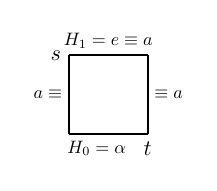
\begin{tikzpicture}[baseline=-0.5ex,
			scale=0.5,
			vdot/.style={rectangle, fill, inner sep=0pt, outer sep=0pt, minimum width=0.5pt, minimum height=6pt},
			dot/.style={draw,fill,circle,inner sep=1.5pt,minimum width=0pt, scale=0.45}
			]
			\draw[thick]
			(0,0) coordinate (a1) -- node[left,scale=0.65]{$a\equiv$} (0,2) coordinate (d1)
			(2,0) coordinate (b1) -- node[right,scale=0.65](q1){$\equiv a$} (2,2) coordinate (c1);
			\draw[thick] (d1) -- node[above,scale=0.65] {$H_1=e\equiv a$} (2,2) coordinate (c1);
			\draw[thick] (a1) -- node[below,scale=0.65] {$H_0=\alpha\quad\;$} (b1);
			\node[below,scale=0.8] at (b1) {$t$};
			\node[left,scale=0.8] at (d1) {$s$};
			\end{tikzpicture} \ar[r]^-H \ar[ru]^-{\widetilde{H}} & \proy^n
		}\]
		
		donde la existencia de $\widetilde{H}$ está garantizada por el lema de elevación (\ref{grf_lema_elevacion_caminos}). 
		
		Ahora, considerando el subconjunto $Z$ formado por los tres lados superiores de $[0,1]\times [0,1]$, tenemos que $\widetilde{H}$ eleva a $e\equiv a$ (en efecto, $p\widetilde{H}=a$). Sin embargo, podemos considerar también la homotopía $\widetilde{H}'=\widetilde{a}$, que es constantemente $\widetilde{a}$. Esta también eleva en $Z$ a $e\equiv a$. Además, coinciden en un punto, pues:
		\[\widetilde{H}_0(0)=\widetilde{\alpha}(0)=\widetilde{a}\]
		y entonces, por la unicidad de la elevación (lema \ref{grf_lema_unicidad_elevacion}), tenemos que $\widetilde{H}=\widetilde{e}$ en $Z$. Pero entonces:
		\[\widetilde{H}_0(1) = \widetilde{\alpha}(1) = \widetilde{e} = \widetilde{a}\]
		pero esto claramente no ocurre por definición de $\widetilde{\alpha}$, luego ya tenemos nuestra contradicción.
		
		Entonces, el grupo fundamental de $\proy^n$ tiene dos elementos, y por tanto tiene que ser $\Z_2$.
	\end{proof}
\end{theo}

\section{El grupo fundamental del círculo}

El objetivo de esta sección es calcular el grupo fundamental de $\Sfe^1$, el círculo de $\R^2$. Además, este es homeomorfo a $\proy^1$, la recta proyectiva real, con lo que, considerando también la sección anterior, ya tendremos el grupo fundamental del espacio proyectivo de cualquier dimensión.

\begin{theo}[Grupo fundamental de $\Sfe^1$]
\label{grf_circulo}

El grupo fundamental de $\Sfe^1$ es $\pi(\Sfe^1)=\Z$.

\begin{proof}
Consideramos el siguiente esquema:
\[\xymatrix @C = 0.5pc {
&&\R \ar[d]^p & t \ar@{|->}[d] \\
[0,1] \ar[rr]^\sigma \ar[rru]^{\widetilde{\sigma}} & & \Sfe^1 & e^{2\pi ti}
}\]
donde ya hemos visto que $\R$ es un espacio recubridor con la aplicación $p$.

Definimos entonces la siguiente aplicación entre grupos:
\[\begin{split}
\indice:\pi(\Sfe^1,a)&\to\Z \\
[\sigma] &\mapsto \indice\sigma = \widetilde{\sigma}(1)-\widetilde{\sigma}(0)
\end{split}\]
para cualquier elevación $\widetilde{\sigma}$ de $\sigma$ en $\R$. La denominamos \tbi[indice@índice]{índice}, \tbi[numero de vueltas@número de vueltas|see{índice}]{número de vueltas} o \tbi[grado|see{índice}]{grado}.

El objetivo de la demostración es comprobar que la aplicación $\indice$ anterior es un isomorfismo de grupos, pues entonces hemos terminado. Desde luego, es necesario comprobar también que está bien definida.

En primer lugar, comprobamos que $\indice$ no depende de la elevación $\widetilde{\sigma}$. Para ello, sea $\widehat{\sigma}$ otra elevación. Tenemos que verificar que $\widetilde{\sigma}(1)-\widetilde{\sigma}(0) = \widehat{\sigma}(1) - \widehat{\sigma}(0)$. Consideramos entonces la aplicación:
\[[0,1]\ni t\mapsto \widetilde{\sigma}(t) - \widehat{\sigma}(t)\]
Como $p\circ\widetilde{\sigma} = p\circ\widehat{\sigma} = \sigma$, necesariamente $\widetilde{\sigma}(t) - \widehat{\sigma}(t)\in\Z$. Dado que la aplicación anterior es continua y $[0,1]$ es conexo, su imagen es conexa, y un conexo en $\Z$ es un punto, es decir, $\widetilde{\sigma}(t) - \widehat{\sigma}(t)$ es constante, y la llamamos $k$. Entonces:
\[\widetilde{\sigma}(1)-\widetilde{\sigma}(0) = (\widehat{\sigma}(1) + k) - (\widehat{\sigma}(0) + k) = \widehat{\sigma}(1) - \widehat{\sigma}(0)\]

Para asegurar que está bien definida, también hace falta ver que $\indice$ no depende del representante. Es decir, que dados $\sigma,\tau$ de forma que $\sigma\homot[a]\tau$, $\indice\sigma = \indice\tau$. Para ello, vamos a recurrir a la elevación: consideramos la homotopía $H:\sigma\homot[a]\tau$. Entonces, tenemos:
\[\xymatrix{
& \R \ar[d]^p \\
[0,1]^2 \ar[ru]^{\widetilde{H}} \ar[r]^-H & \Sfe^1
}\]
donde la existencia de la elevación $\widetilde{H}$ está garantizada por el lema de elevación de homotopías (\ref{grf_lema_elevacion_homotopias}). Está claro que $\widetilde{H}_0 = \widetilde{\sigma}$ y $\widetilde{H}_1 = \widetilde{\tau}$. Además, por ser $H$ homotopía con el extremo $a$ fijo, para todo $s$ $H_s$ es un lazo con base $a$.

Ahora, como queremos ver que $\indice\sigma = \indice\tau$, consideramos la aplicación $s\mapsto \widetilde{H}_s(1)-\widetilde{H}_s(0)=\indice(H_s)$, que está bien definida por ser cada $H_s$ un lazo. Entonces, está claro que $\indice(H_s)\in\Z$, y por ser una aplicación de $[0,1]$ en $\Z$ continua, es constante. Entonces:
\[\indice\sigma = \indice(H_0) = \indice(H_1) = \indice\tau\]

Así, ya hemos visto que está bien definida. Falta comprobar pues que es biyectiva y homomorfismo de grupos.

Desde luego, es sobreyectiva. En efecto, consideramos los caminos $[0,1]\ni t\mapsto e^{2k\pi it}$, con $k\in\Z$.  Entonces, cada uno de ellos tiene una elevación $\widetilde{\sigma}(t)=kt$, de forma que su índice es $k$.

Para ver la inyectividad, hay que comprobar que $\indice\sigma = \indice\tau\implies \sigma\homot[a]\tau$. Podemos escoger un par de elevaciones $\widetilde{\sigma},\widetilde{\tau}$ que verifiquen que $\widetilde{\tau}(0)=\widetilde{\sigma}(0)$. Así, como $\indice\sigma = \widetilde{\sigma}(1)-\widetilde{\sigma}(0)$, $\indice\tau = \widetilde{\tau}(1)-\widetilde{\tau}(0)$, y son iguales, resulta que $\widetilde{\sigma}(1)=\widetilde{\tau}(1)$.

Ahora, está claro que la interpolación lineal $(1-s)\widetilde{\sigma}(t) + s\widetilde{\tau}(t)$ es una homotopía en $\R$. Entonces, $H_s \coloneqq p((1-s)\widetilde{\sigma}(t) + s\widetilde{\tau}(t))$ es una homotopía en $\Sfe^1$ entre $\widetilde{\sigma}$ y $\widetilde{\tau}$. Pero aún falta probar que es homotopía de lazos. En efecto:
\[H_s(0)= p((1-s)\widetilde{\sigma}(0) + s\widetilde{\tau}(0))=p(\widetilde{\sigma}(0))=\sigma(0)=a\]
\[H_s(1)= p((1-s)\widetilde{\sigma}(1) + s\widetilde{\tau}(1))=p(\widetilde{\sigma}(1))=\sigma(1)=a\]

Por fin, ya solo falta ver que $\indice$ es homomorfismo de grupos. Como el grupo fundamental se definía con la operación $\pathp$, de forma que $[\sigma]\pathp[\tau]=[\sigma\pathp\tau]$, tenemos que verificar que $\indice\sigma + \indice\tau = \indice(\sigma\pathp\tau)$.

Entonces, volviendo a la definición de índice, tenemos que:
\[\indice\sigma = \widetilde{\sigma}(1)-\widetilde{\sigma}(0)\]
\[\indice\tau = \widetilde{\tau}(1)-\widetilde{\tau}(0)\]
\[\indice(\sigma\pathp\tau) = \widetilde{\sigma\pathp\tau}(1)-\widetilde{\sigma\pathp\tau}(0)\]
donde podemos escoger $\widetilde{\tau}(0)=\widetilde{\sigma}(1)$, de forma que $\widetilde{\sigma}\pathp\widetilde{\tau}$ esté bien definido. Entonces, este es un camino de $\widetilde{\sigma}(0)$ a $\widetilde{\tau}(1)$, es decir, de $a$ a $a$.

Como $p\circ(\widetilde{\sigma}\pathp\widetilde{\tau}) = \sigma\pathp\tau$, sabemos que $\widetilde{\sigma}\pathp\widetilde{\tau} = \widetilde{\sigma\pathp\tau}$, por unicidad de la elevación. Entonces:
\[\indice(\sigma\pathp\tau)=\widetilde{\sigma\pathp\tau}(1)-\widetilde{\sigma\pathp\tau}(0)=\widetilde{\tau}(1)-\widetilde{\sigma}(0)=\widetilde{\tau}(1)-\widetilde{\tau}(0) + \widetilde{\sigma}(1)-\widetilde{\sigma}(0)=\indice\sigma + \indice\tau\]
como queríamos.
\end{proof}
\end{theo}

\begin{cor}[Grupo fundamental de $\proy^1$]
El grupo fundamental de \indexg{espacio proyectivo} $\proy^1$ es $\pi(\proy^1)=\Z$.

\begin{proof}
Trivial por ser $\proy^1\homeo\Sfe^1$. 
\end{proof}
\end{cor}

\begin{cor}[Grupo fundamental del toro]
El grupo fundamental del toro de revolución $\toro$ es $\pi(\toro)=\Z^2$.

\begin{proof}
Como el toro \indexg{toro@toro de revolución} es homeomorfo a $\Sfe^1\times\Sfe^1$, la proposición \ref{grf_prop_gf_prod_es_prod_gf} nos asegura que:
\[\pi(\toro)=\pi(\Sfe^1)\times\pi(\Sfe^1)=\Z^2\]
\end{proof}
\end{cor}

\begin{cor}
El grupo de rotaciones \indexg{SO(3)} $SO(3)$ no es homeomorfo a $\Sfe^1\times\Sfe^2$.

\begin{proof}
En efecto, se puede comprobar (aunque no lo haremos aquí) que $SO(3)\homeo\proy^3$. Por tanto, como ya vimos en el teorema \ref{grf_espacio_proyectivo}, tiene grupo fundamental $\Z_2$. Sin embargo, $\Sfe^1\times\Sfe^2$ tiene por grupo fundamental $\Z$, por el resultado anterior.
\end{proof}
\end{cor}

\section{Retractos de deformación}

Ya comentamos en su momento el concepto de retracto. En esta sección vamos a presentar un tipo especial de retracto, el retracto de deformación, que tiene una importancia capital, pues respeta el grupo fundamental.

Empezamos dando formalmente la definición de retracto:

\begin{defi}[Retracto]
	Un \tbi{retracto} del espacio $\X$ es un subespacio $A\subset\X$ tal que existe una aplicación continua $\rho:\X\to A$ que deforma el espacio en él, de forma que $\rho\restriction_A = \Id_A$.
\end{defi}

Y pasamos directamente a definir lo que verdaderamente nos importa.

\begin{defi}[Retracto de deformación]
	Un subespacio $A\subset\X$ es un \tbi[retracto!de deformación]{retracto de deformación} si es un retracto, con aplicacion $\rho$, y existe una homotopía que verifique:
	\[H_s:\X\to\X\left\{\begin{array}{l}
	H_0 = \Id_\X \\
	H_1 = \rho:\X\to A \\
	H_s\restriction_A = \Id_A
	\end{array}\right. \]
\end{defi}

Intuitivamente, un retracto de deformación es un subespacio $A\subset\X$ al que podemos deformar $\X$ ``sin salirnos'' del espacio, y, además, ``sin mover'' $A$.

\begin{obs}[Interpolación lineal]
	\label{grf_obs_interpolacion_retractos}
	Dado un retracto con aplicación $\rho:\X\to A$, se define:
	\[H_s(x) = (1-s)x+s\rho(x)\]
	si es posible, es decir, si el segmento $[x,\rho(x)]\subset\X$ para cada $x\in\X$. En el caso de que se pueda definir, $A$ es retracto de deformación de $\X$.
\end{obs}

\begin{exa}
	Listamos ahora una serie de retractos de deformación que podemos construir:
	\begin{enumerate}
		\item $\Sfe^{n-1}$ es retracto de $\R^n\setminus\{0\}$, a través de la aplicación:
		\[\begin{split}
		\rho: \R^n\setminus\{0\} &\to\Sfe^{n-1} \\
		x &\mapsto\frac{x}{\norm{x}}
		\end{split}\]
		
		Además, se verifica la condición de la observación \ref{grf_obs_interpolacion_retractos}, con lo cual es retracto de deformación.
		
		\item $\Sfe^1$ es retracto de deformación del cilindro $C$. En efecto, escribimos directamente la homotopía:
		\[H_s(x,y,z)=(1-s)(x,y,z) + s(x,y,0)\]
		que induce un retracto de deformación.
		
		\item Una circunferencia es retracto de deformación de una banda de Möbius.
		% TODO: dibujo?
		
		\item La lemniscata (el bouquet con dos círculos) es retracto de deformación de $\R^2\setminus\{a,b\}$. \qedhere
		% TODO: dibujo?
	\end{enumerate}
\end{exa}

Los espacios que pueden retraerse a un punto son especialmente interesantes:

\begin{defi}
	Sea $a\in\X$. Decimos que $\X$ es \tbi{contráctil} si $\{a\}$ es retracto de deformación de $\X$.
\end{defi}

Pasamos pues al resultado fundamental de esta sección:

\begin{theo}
	Si $A\subset\X$ es un retracto de deformación con aplicación $\rho$, entonces:
	\[\rho^*:\pi(\X,a)\to\pi(A,a)\]
	es isomorfismo. En consecuencia, $\X$ y $A$ tienen el mismo grupo fundamental.
	
	\begin{proof}
		Hay que comprobar que es isomorfismo:
		\begin{itemize}
			\item Es homomorfismo por definición de $\rho^*$.
			\item Es sobreyectivo por ser retracto, como ya vimos en la proposición \ref{grf_prop_retractos_homo_sobreyectivo}.
			\item Es inyectivo. En efecto, consideramos un lazo $\sigma$ con base $a$, y el esquema:
			\[\xymatrix{
				[0,1] \ar[r]^\sigma \ar[rd]_{\rho\circ\sigma} & \X \ar[d]^\rho \\
				& A
			}\]
			
			Como sabemos, el homomorfismo $\rho^*$ manda $[\sigma]\mapsto [\rho\circ\sigma]$. Para ver la inyectividad, basta ver que el núcleo es trivial. Entonces, si $[\rho\circ\sigma] = 1$, existe una homotopía $F_s:\rho\circ\sigma\homot[a] e$.
			
			Llamando $H_s$ a la deformación, definimos la homotopía $G_s=H_s\circ\sigma$. Entonces, se verifica:
			\begin{gather*}
				H_0\circ\sigma= \sigma \homot H_1\circ\sigma = \rho\circ\sigma \\
				H_s\circ\sigma(0) = H_s\circ\sigma(1) = H_s(a) = a
			\end{gather*}
			y entonces $\sigma$ es homótopo a $\rho\circ\sigma$, pero este a su vez es homótopo a una constante. Entonces, el núcleo es trivial. \qedhere  
		\end{itemize}
	\end{proof}
\end{theo}